
% ==============================================================================
% SECTION 4: ACCIDENT DE DESATURATION (ADD)
% ==============================================================================
\section{L'Accident de Désaturation (ADD)}

\begin{frame}{Attentes pédagogiques N3 — ADD}
    Dans le cadre de leurs nouvelles prérogatives, les plongeurs N3 évoluent jusqu'à \textbf{60 mètres}.\\
    Cette zone profonde accroît les risques ; les connaissances en prévention, organisation et secours doivent donc être approfondies.

    \vspace{1em}
    À propos de l'\textbf{accident de décompression}, le futur Niveau 3 doit :
    \begin{itemize}
        \item Connaître les \textbf{causes}.
        \item Identifier les \textbf{symptômes} pour le détecter en l'absence de Guide de Palanquée (GP).
        \item Savoir le \textbf{prévenir}.
        \item Maîtriser la \textbf{Conduite à Tenir (CAT)}.
        \item Être capable de répondre aux questions (écrites/orales) de l'examen.
    \end{itemize}
\end{frame}

\begin{frame}{Mécanisme de l'ADD — Principe}
    \begin{block}{Principe Physique : Loi de Henry}
        À température constante, la quantité de gaz dissous dans un liquide est proportionnelle à la pression au-dessus du liquide.
        \[ \text{Quantité de gaz} = \text{Coefficient} \times \text{Pression} \]
    \end{block}

    \vspace{1em}
    \textbf{Le problème en plongée :}
    \begin{itemize}
        \item À la descente, l'azote se dissout dans les tissus (\textbf{sous saturation}).
        \item À la remontée, la pression diminue, l'azote doit être évacué.
        \item Si la remontée est \textbf{trop rapide} ou l'élimination perturbée, des bulles se forment (effet bouteille de champagne) et bloquent la circulation.
    \end{itemize}
\end{frame}

\begin{frame}{Rappels de Physiologie — Échanges Gazeux}
    \begin{columns}[T,totalwidth=\textwidth]
        \column{0.5\textwidth}
        \centering
        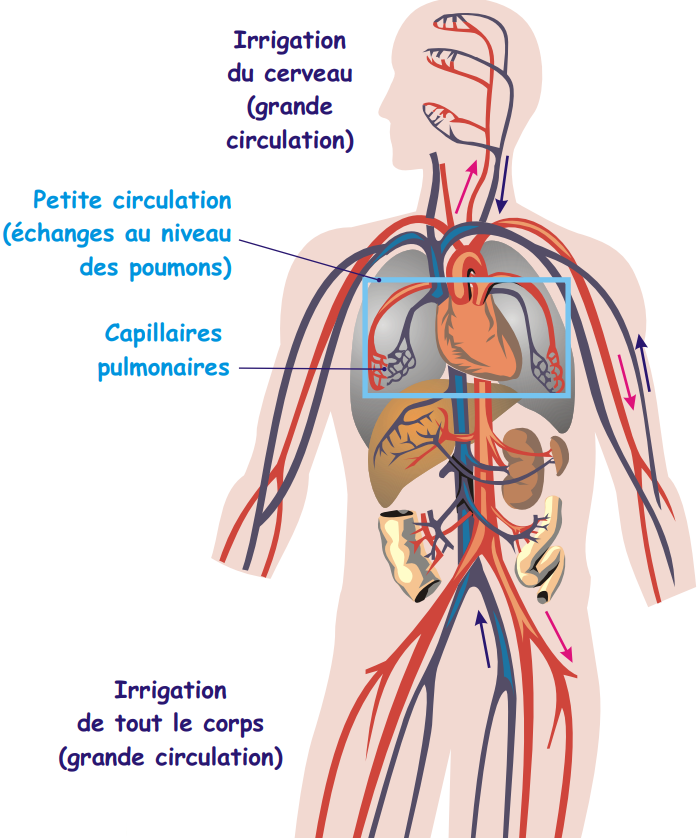
\includegraphics[height=0.85\textheight]{images/add_circulation.png}

        \column{0.5\textwidth}
        \small
        \textbf{\textcolor{ffessmred}{Oxygène ($O_2$)}} \\
        Carburant de l'organisme, inspiré via l'air.
        
        \vspace{0.8em}
        \textbf{\textcolor{ffessmred}{Dioxyde de Carbone ($CO_2$)}} \\
        Déchet du travail musculaire, éliminé à l'expiration.
        
        \vspace{0.8em}
        \textbf{Mécanisme}
        \begin{itemize}
            \item \textbf{Échanges} gazeux (O$_2$/CO$_2$/N$_2$) au niveau des \textbf{alvéoles pulmonaires}.
            \item \textbf{Transport} : Le sang véhicule les gaz entre les poumons et toutes les cellules via le \textbf{système circulatoire}.
        \end{itemize}
    \end{columns}
\end{frame}

% --- DÉFINITIONS GLOBALES ---
% (À laisser ici ou dans le préambule de main.tex)
\tikzset{
    box_double/.style={
        rectangle split,
        rectangle split parts=2,
        rectangle split part fill={yellow, white},
        draw=black, thick,
        align=center,
        minimum width=1.8cm,
        minimum height=1.6cm
    },
    star_alert/.style={
        star, star points=9, star point ratio=1.4,
        draw=red, fill=red, text=black,
        align=center, font=\bfseries\scriptsize,
        inner sep=2pt
    },
    arrow/.style={->, >=Latex, thin, black},
    bubble/.style={
        ellipse, draw=black, fill=white,
        align=center, font=\scriptsize, inner sep=2pt
    }
}

\newcommand{\drawstate}[5]{
    \node[box_double] (#1) at (#2, #3) {
        #4
        \nodepart{two}
        #5
    };
}

\begin{frame}{Le mécanisme de saturation}
    \centering
    
    \begin{tikzpicture}[
        scale=0.5, transform shape,
        font=\sffamily\bfseries
    ]

    % --- A. LE PROFIL ---
    \draw[line width=2pt] 
        (-2, 0) -- (-1, 0)       % DEPART : Une ligne horizontale en surface (de gauche à droite)
        -- (2, -6)              % DESCENTE : On descend jusqu'à Y=-6 (le fond)
        -- (9, -6)              % FOND : On reste à -6 jusqu'à X=8 (ligne plate)
        -- (11, -4)             % REMONTÉE : On remonte jusqu'à -4 (premier palier)
        -- (13, -4)             % PALIER 1 : On reste stable à -4 pendant 2 unités
        -- (14, -2)             % REMONTÉE : On remonte jusqu'à -2 (deuxième palier)
        -- (16, -2)             % PALIER 2 : On reste stable à -2
        -- (17, 0) -- (20, 0);  % SORTIE : On remonte en surface (0) et on nage un peu.
    \draw[line width=2pt, dashed] (11, -4) -- (12, 1);

    % --- B. LES ÉTATS ---
    \drawstate{s1}{2}{1}{++}{++}
    \node[left=0.2cm of s1, align=right] {Saturation};

    \drawstate{s2}{2}{-3}{++++}{++}
    \node[left=1cm of s2, align=right] {Sous\\Saturation};

    \drawstate{s3}{3.5}{-7.5}{++++++}{++++}
    \node[left=0.2cm of s3, align=right] {Sous\\Saturation};
    
    \drawstate{s4}{7.5}{-7.5}{++++++}{++++++}
    \node[below=0.2cm of s4] {Saturation};
    
    \drawstate{s5}{11}{-3}{++++}{+++++}

    \drawstate{s6}{15}{-1}{+++}{+++++}
    \node[right=0.5cm of s6] {Sur-Saturation};

    \drawstate{s7}{18}{1}{++}{++++}
    \node[right=0.2cm of s7] {Sur-Saturation};

    % --- 7. ACCIDENT ---
    % 1. On dessine D'ABORD la boîte s7 pour qu'elle existe
    \drawstate{s8}{12}{1}{++}{+++++}
    
    % 2. On dessine l'étoile DERRIÈRE (sur le calque 'background')
    % Cela nécessite \usetikzlibrary{backgrounds} dans main.tex
    \begin{scope}[on background layer]
        \node[star_alert, fit=(s8), scale=1] {}; 
    \end{scope}

    \node[right=0.1cm of s8, align=left, font=\bfseries\tiny] {Sur-Saturation\\Critique !!!};


    % --- C. FLÈCHES ---
    \draw[arrow] (s1.south) -- (s2.north);
    \draw[arrow] (s2.south) -- (s3.north);
    \draw[arrow] (s3.east) -- (s4.west);
    \draw[arrow] (s4.north) -- (s5.south);
    \draw[arrow] (s5.north) -- (s8.south);
    \draw[arrow] (s5.north) -- (s6.south);
    \draw[arrow] (s6.north) -- (s7.south);

    % --- D. LÉGENDE ---
    \node[bubble, fill=yellow, text width=2cm] (explYellow) at (13, -5.5) 
        {Pression\\partielle\\de N2\\dans l'air\\respiré};
    \node[bubble, text width=2.5cm] (explWhite) at (16, -7) 
        {N2 dissous\\dans le corps\\du plongeur};

    \draw[->, thin] (explYellow) -- (s4.one east);
    \draw[->, thin] (explWhite) -- (s4.two east);

    \end{tikzpicture}
\end{frame}

\begin{frame}{Cause et Mécanismes de l'ADD — Synthèse}
    \textbf{\textcolor{ffessmred}{Mécanismes}} :
    \begin{enumerate}
        \item \textbf{Reprise gazeuse} : À la remontée (baisse de pression), l'azote stocké repasse à l'état gazeux.
        \item \textbf{Évacuation} : Il quitte les tissus vers le sang, direction les poumons pour être expiré.
        \item \textbf{Blocage} : Si l'évacuation est perturbée (mauvais comportement, bulles trop volumineuses), l'azote s'accumule et \textbf{bloque la circulation}.
        \item \textbf{Conséquence} : Les tissus en aval ne sont plus oxygénés, occasionnant des \textbf{dommages} divers.
    \end{enumerate}

    \vspace{0.8em}

    \textbf{\textcolor{ffessmred}{Cause}} :
    \begin{itemize}
        \item \textbf{Blocage} de la circulation par des \textbf{\textcolor{ffessmred}{bulles d'azote}} dans le système sanguin lors de la désaturation.
    \end{itemize}
\end{frame}

\begin{frame}{Prévention de l'ADD — Principes Généraux}
    La prévention ne se limite pas au respect des tables.
    
    \begin{itemize}
        \item \textbf{Objectif} : Minimiser autant que possible les \textbf{\textcolor{ffessmred}{facteurs favorisants}}.
        \item \textbf{Responsabilité N3} : En autonomie, vous devez être particulièrement attentif pour \textbf{\textcolor{ffessmred}{modérer sa plongée}}.
        \item \textbf{Stratégie} : Limiter la \textbf{\textcolor{ffessmred}{charge en azote}} pour aller dans le sens de la sécurité.
    \end{itemize}

    \vspace{0.5em}
    \begin{block}{Règle d'or}
        Adopter un comportement adéquat \textbf{Avant}, \textbf{Pendant} et \textbf{Après} la plongée.
    \end{block}
\end{frame}

\begin{frame}{Prévention — Avant et Pendant}
    \textbf{Avant la plongée} :
    \begin{itemize}
        \item Ne pas plonger si \textbf{\textcolor{ffessmred}{fatigué}} ou sans envie.
        \item Vérifier la compatibilité des \textbf{\textcolor{ffessmred}{traitements médicaux}}.
    \end{itemize}

    \vspace{0.5em}
    \textbf{Pendant la plongée} :
    \begin{itemize}
        \item \textbf{\textcolor{ffessmred}{Effort}} et \textbf{\textcolor{ffessmred}{Froid}} : À limiter impérativement (augmentent la saturation).
        \item \textbf{\textcolor{ffessmred}{Profil}} : Éviter les profils \textbf{\textcolor{ffessmred}{Yoyo}} ou \textbf{\textcolor{ffessmred}{Inversés}}.
        \item \textbf{\textcolor{ffessmred}{Vitesse}} : Respect strict de la vitesse de remontée.
        \item \textbf{\textcolor{ffessmred}{Valsalva}} : Ne jamais faire de manœuvre force/prolongée à la remontée (gêne l'élimination pulmonaire).
    \end{itemize}
\end{frame}

\begin{frame}{Prévention — Après et Facteurs Individuels}
    \textbf{Après la plongée} (La désaturation continue en surface !) :
    \begin{itemize}
        \item Pas d'\textbf{\textcolor{ffessmred}{effort}} intense ("Sport" après plongée).
        \item Pas d'\textbf{\textcolor{ffessmred}{apnée}} (perturbe les échanges, attendre \textbf{au moins 6h}).
        \item Pas d'\textbf{\textcolor{ffessmred}{altitude}} (Montagne/Avion) : Planifier sa journée.
    \end{itemize}
    
    \vspace{0.5em}
    \textbf{Facteurs Physiologiques} (Facteurs de risque intrinsèques) :
    \begin{itemize}
        \item L'\textbf{\textcolor{ffessmred}{âge}}, la forme physique (surpoids).
        \item Le \textbf{\textcolor{ffessmred}{tabagisme}} (mauvaise vascularisation).
        \item L'\textbf{\textcolor{ffessmred}{alcool}}, la drogue, les médicaments.
    \end{itemize}
\end{frame}

\begin{frame}{Symptômes de l'ADD}
    Peuvent apparaître dès la sortie ou plusieurs heures après.
    
    \begin{alertblock}{Signes d'alerte}
        \begin{itemize}
            \item \textbf{Fatigue intense} (anormale).
            \item Troubles cutanés ("Puces", moutons).
            \item Troubles neurologiques : Fourmillements, paralysies, troubles sensitifs (vue, ouïe).
            \item Vertiges, nausées.
            \item Douleurs articulaires.
        \end{itemize}
        \textbf{\textcolor{ffessmred}{Règle d'or}} : Toute sensation anormale ou trouble (douleur dos, élocution, prostration...) 
        doit être \textbf{\textcolor{ffessmred}{considérée avec sérieux}} et traitée comme un ADD.
    \end{alertblock}
    \textit{Surveillance mutuelle impérative après la plongée !}
\end{frame}


\begin{frame}{Conduite à Tenir (CAT) - RIFAP}
    En l'absence de DP, le N3 prend en charge les secours :
    
    \begin{enumerate}
        \item \textbf{Sortir et Allonger} la victime (ne pas surélever les jambes).
        \item \textbf{Oxygène pur} : Inhalation à 15 L/min (le plus tôt possible).
        \item \textbf{Hydratation} : Faire boire de l'eau plate (si conscient) $\sim$ 1 Litre.
        \item \textbf{Alerte} : CROSS, Pompiers ou le SAMU.
        \item \textbf{Évacuation} : Organiser le transfert vers un caisson hyperbare.
        \item \textbf{Fiche d'évacuation} : Noter les paramètres de la plongée pour les médecins.
        \item \textbf{Surveillance} : Mettre à l'ombre, couvrir la victime et maintenir une surveillance.
    \end{enumerate}
\end{frame}
